\documentclass[12pt]{article}

% Language setting
\usepackage[utf8]{inputenc}
\usepackage[bulgarian]{babel}

% --------------------- Packages  --------------------
% Use biblatex
\usepackage{biblatex}
\addbibresource{bibliography.bib}
% Table thickness
\usepackage{ctable}
% Equations: SI units
\usepackage{siunitx}
% Approximately equal
\usepackage{amssymb}
% degrees symbol
\usepackage{gensymb}
% warning box
\usepackage{pifont,mdframed}

\newenvironment{warning}
  {\par\begin{mdframed}[linewidth=2pt, linecolor=white]%
    \begin{list}{}{\leftmargin=1cm
                   \labelwidth=\leftmargin}\item[\Large\ding{43}]}
  {\end{list}\end{mdframed}\par}

% --------------------- Title  --------------------
\addbibresource{bibliography.bib}

% Acronyms
\usepackage[acronym]{glossaries}
\makeglossaries
\newacronym{me}{МЕ}{модул на еластичност}

\begin{document}

% Anfang der Titelseite________________________________________________________________________________
\begin{titlepage}
	\flushleft
% 	\begin{center}
	%{\scshape\Large Werkstoffe III \hspace{2.5cm} Laborbericht \hspace{&2.5cm}HS 2022 \par}
	{\scshape\Large Протокол VI \hspace{2cm} Механика - практикум\par}
	\vspace{5cm}
	{\huge\bfseries Еластичност при огъване и при усукване\par}
	\vspace{1cm}
	{\LARGE\bfseries Лабораторно упражнение №14\par}
	\vspace{5cm}
    % {\LARGE\bfseries Физически Факлутет към Софийски Университет ``Св. Климент Охридски \par}
    {\LARGE\bfseries Виолета Кабаджова, \par}
%   {\LARGE\bfseries Group: X\par}
    {\large\bfseries ККТФ, фак. номер: 3PH0600026\par}
	\vspace{1cm}
	
	{\large Физически Факултет, 
	
	Софийски Университет "Св. Климент Охридски"
	
	15 ноември 2022 г.\par}
	
\end{titlepage}

\section{Теоритична част}\label{sec:theoretical-part}

\printglossary[type=\acronymtype,title={Използвани съкращения}]

\subsection{Видове деформация и модули на еластичност}
Деформация е всяка промяна в обема и/или формата на тяло. Тя може да бъде еластична или пластична в зависимост от това до колко тялото възстановява изходното си състояние след деформацията, като идеално еластична деформация е такава, при която тялото възстановява геометриите си напълно, а идеално пластична - изобщо. Също така деформацията може да бъде хомогенна или нехомогенна спрямо това дали всички елементарни обеми се деформират еднакво или не.

Видът на деформацията зависи от вида и свойствата на материала, както и от големината на приложената сила в съответната единица площ (механично напрежение). Различните видове деформации описваме чрез т.нар. модули на еластичност [$N/m^2$], стойностите на които са характерни за съответните конкретни материали.

Големината на една деформация зависи както от модула на еластичност, така и от геометрията на съответните тела (форми и размери), които биват поставени под деформация.

\subsection{I модул на еластичност Е (Модул на Юнг)}
На фиг. \ref{fig:stretching} е илюстрирана деформация при опъване. Началната дължина на тялото бележим с $l$, а деформираната - $l_0$. 

Съгласно закона на Хук при малки еластични деформации относителната деформация $\varepsilon = \frac{|\Delta l|}{l_0} = \frac{|l - l_0|}{l_0}$ зависи линейно от приложеното механично напрежение, а единица върху този коефициент наричаме модул на Юнг.

\begin{equation}
    \varepsilon = \alpha \tau_n = \alpha \frac{F}{S}
\end{equation}

\begin{equation}
    E = \frac{1}{\alpha}
\end{equation}

Оттук можем да заключим, че модулът на Юнг е равен на нормалното механично напрежение F, което трябва да се приложи към тялото, за да се получи удължение $\varepsilon$, равно на първоначалния му размер, ако все още е в сила законът на Хук:

\begin{equation}
    \varepsilon = \frac{|\Delta l|}{l_0} = \frac{\tau_n}{E} = \frac{1}{E} \frac{F}{S}
\end{equation}

\begin{equation}
    E = \varepsilon \frac{F}{S}
\end{equation}


\begin{figure}
    \centering
    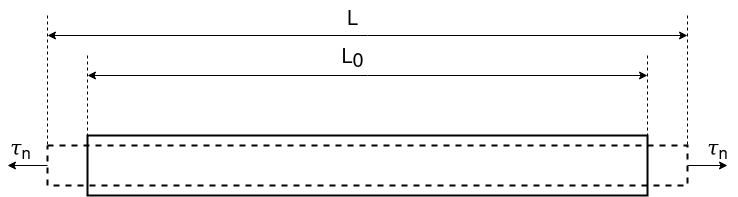
\includegraphics[width=1\textwidth]{images/young.drawio.png}
    \caption{Деформация на едноосно опъване}
    \label{fig:stretching}
\end{figure}

\subsection{II модул на еластичност $\Phi$}
Втори модул на еластичност (или още модул на еластичност при хлъзгане) наричаме $\Phi = \frac{1}{\gamma}$, където $\gamma$ е коефициентът на еластичност при хлъзгане при прилагане на тангенциално механично напрежение $\tau_t = \frac{F}{S}$ за еластични деформации при малки ъгли $\psi$ (виж фиг. \ref{fig:second-modulus-of-elasticity}). Тогава: 

\begin{equation}
    tg\psi = \psi = \frac{\Delta l}{l_0} = \gamma \tau_t = \frac{1}{\Phi} \tau_t
\end{equation}

\begin{figure}
    \centering
    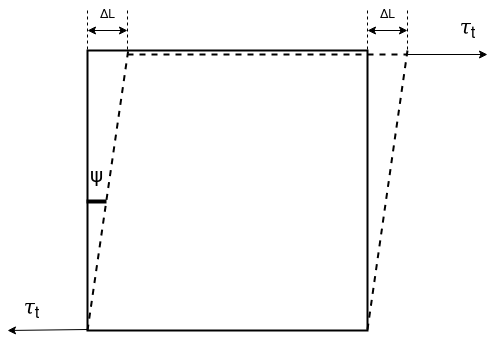
\includegraphics[width=0.5\textwidth]{images/yound-second-modulus.drawio.png}
    \caption{Хомогенен куб със страна $l_0$ и стена с площ S, чиято долна основа е неподвижно закрепена и върху който бива проложенио тангенциално механично напрежение $\tau_t = \frac{F}{S}$}
    \label{fig:second-modulus-of-elasticity}
\end{figure}

$\Phi < E$ за всеки материал.

\section{Експериментална част}
\subsection{Деформация при огъване и деформация при усукване}
Нехомогенните дефорамции на огъване и усукване можем да сведем до хомогенни, представяйки деформациите по слоевете на елементарните обеми.

На фиг. \ref{fig:bending} е представена пластина при огъване, част от слоевете на които са подложени на опън (в изпъкналата ѝ страна), а друга част - на свиване (във вдлъбнатата ѝ страна). Съществува и "неутрален" слой, който запазва първоначалната си дължина $l_0$. При приложено напрежение в средата между опорните точки, на които е подпряна пластината, преместването $\Delta h$ се изразява чрез:

\begin{equation}\label{eq:delta-h}
    \Delta h = \frac{l_0^3}{4Ea^3b}G,
\end{equation}

където $a$ и $b$ са съответно дебелината и ширината на пластината, а $\Vec{G} = m\Vec{g}$.

\begin{figure}
    \centering
    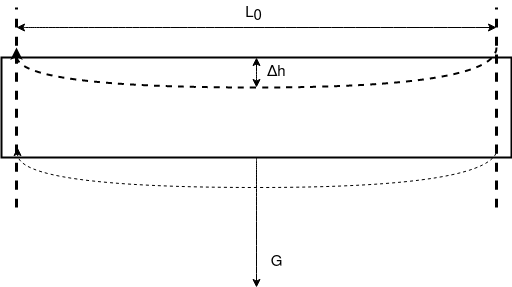
\includegraphics[width=0.5\textwidth]{images/young-bending.drawio.png}
    \caption{Деформация при огъване}
    \label{fig:bending}
\end{figure}

Деформацията при усукване (торзия) от своя страна може да се опише чрез деформация при хлъзгане (т.е. с втория модул на еластичност $\Phi$). Може да се пресметне, че вторият модул на еластичност за нехомогенна цилиндрична пръчка с радиус $R$ и дължина $l$, която се усуква на ъгъл $\phi$ под действие на момента на фвойка сили $(\Vec{F}, \Vec{F})$ е:

\begin{equation}\label{eq:phi-modulus}
    \Phi = \frac{2l}{\pi R^4 \phi}M,
\end{equation}

където $M$ е момента на двойката сили, която е $M=2FR$.
\subsection{Задача: Измерване на модула на Юнг Е чрез деформация при огъване на планстина}

Експерименталната установката е подобна на показаната на фиг. \ref{fig:bending} - пластина е поставена върху две опорни точки, като последователно се поставят тежести в средата на дължината. След поставянето на всяка от тежестите се измерва новата стойност на височината на средата на пластината и се изчислява $\Delta h_i$. 

Тъй като в работната формула за пресмятане на модула на Юнг, дебелината $a$ на пластината е повдигната на трета степен, я измерваме няколкократно, за да вземем средна стойност и да намалим грешката в последствие. Същото правим и за ширината $b$, а резултатите записваме в таблица \ref{tbl:length-width}.

\begin{table}[h]
\begin{center}
\begin{tabular}{|l|l|l|}\hline
N	&a_i, [mm]	&b_i, [mm] \\ \hline
1	&0.148	&2.42\\ \hline
2	&0.13	&2.461\\ \hline
3	&0.13	&2.431\\ \hline
4	&0.16	&2.443\\ \hline
\specialrule{.1em}{0em}{0em}
&$\bar{a}$ = 0.142 &$\bar{b}$ = 2.439\\ \hline
\end{tabular}
\caption{\label{tbl:length-width}Измерване на дебелината и ширината в различни части от пластината}
\end{center}
\end{table}

Получените резутати са представени в таблица \ref{tbl:delta-h}, където $\Delta m_i$ и $\Delta m_i '$ представляват съответно добавената и премахнатата допълнителна маса на всяка итерация, $m_i$ и $m_i '$ са общата добавена и премахната маса (кумулативна стойност). $h_i$ и $h_i'$ са измерените височини на средата на пластината в съответния момент след извършване на промяна по общата маса, оказваща механично напрежение, а $\Delta h_i$ и $\Delta h_i'$ - пресметнатата кумулативна стойност за промяна на височината (т.е. общата стойност на промяната).

Използвайки формула \ref{eq:e_i} като следствие от формула \ref{eq:delta-h}`, пресмятаме $E_i$ на всяка итерация, след което пресмятаме и средната стойност $\Bar{E}$, като записваме резултатите в същата таблица. 
\begin{equation}\label{eq:e_i}
    E_i = \frac{l_0^3}{4a^3b\Delta h_i}G,
\end{equation}

\begin{table}[h]
\begin{center}
\begin{tabular}{|l|l|l|l|l|l|}\hline
\multicolumn{5}{c}{Добавяне на тежести} \\ \hline
N &\Delta m_i, [g] &m_i, [g] &h_i, [mm] &\Delta h_i, [mm] &E_i \cdot 10^{12} [N/m^2] \\ \hline
0 &0 &0 &18.96 &0 & -\\\hline
1 &100.89 &100.89 &17.1 &1.86 & 189.02 \pm 80.17 \\\hline
2 &99.95 &200.84 &15.714 &3.25 & 215.62 \pm 91.45\\\hline
3 &102.46 &303.3 &14.164 &4.80 & 220.38 \pm 93.48\\\hline
4 &102.25 &405.55 &12.591 &6.37 & 221.90 \pm 94.13 \\\hline
&       &       &       &      &$\bar{E} = 211.73 \pm 89.80$\\ \hline
\multicolumn{5}{c}{Премахване на тежести} \\ \hline
N &\Delta m\_i', [g] &m_i'&h_i', [mm] &\Delta h_i', [mm] &E_i \cdot 10^{12} [N/m^2] \\ \hline
0 &0 &405.55 &12.591 &- & -\\\hline
1 &102.25 &303.3 &14.146 &4.81 & 219.56 \pm 93.13 \\\hline
2 &102.46 &200.84 &15.684 &3.28 & 213.64 \pm 90.61 \\\hline
3 &99.95 &100.89 &17.05 &1.91 & 184.08 \pm 78.07\\\hline
4 &100.89 &0 &18.88 &0.08 & - \\\hline
&       &       &       &      &$\bar{E}' = 205.76 \pm 87.27$\\ \hline
\end{tabular}
\caption{\label{tbl:delta-h}Изчисляване на $\Delta h_i$ за всяка добавена тежест. Втората половина на таблицата съдържа обратното действие - премахване на тежестите една по една и изчисляването на \Delta h_i'}
\end{center}
\end{table}

За първата и последната стойност не можем да измерим $E_i$, тъй като референтната стойност, спрямо която изчисляваме $\Delta h_i$ е именно стойността на височината на съответния ред. При добавянето на тежестите референтната ни стойност е тази, при която няма сложена никаква тежест, а именно - измерване 0. При премахването на тежестите, за референтна взимаме стойността, при която всички тежести са сложени, т.е. последната стойност на добавена тежест в първата част от таблицата - $h_4$. Въпреки това стойността на $E_3$ в последния ред на втората част от таблицата, не може да бъде пресметнат, защото общата допълнителна маса, приложена върху пластината, е равна на 0, което занулява цялата стойност съгласно формула \ref{eq:e_i}.

Оглеждайки таблиците, виждаме, че модулите между всеки две двойки от всяка от таблиците са равни в рамките на абсолютната си грешка. Същото се отнася и за стойностите между двойките от двете таблици (т.е. модулът на Юнг при добавяне на тежест е същият като при разтоварване).


Графиката на зависимостта $\Delta h(m_i)$ е илюстрирана на фиг. \ref{fig:dataanal}.

\begin{figure}
    \centering
    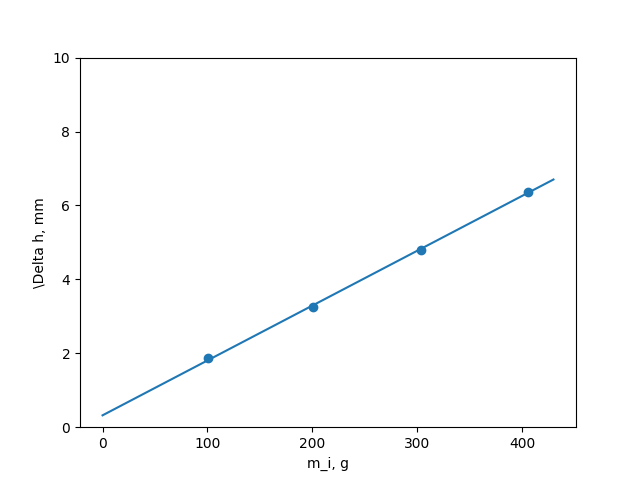
\includegraphics[width=1\textwidth]{images/dataanal.png}
    \caption{Построяване на графиката \Delta h(m_i)}
    \label{fig:dataanal}
\end{figure}


\section{Задача: Измерване на втория модул на еластичност чрез деформация на усукване на пръчка}


\begin{figure}
    \centering
    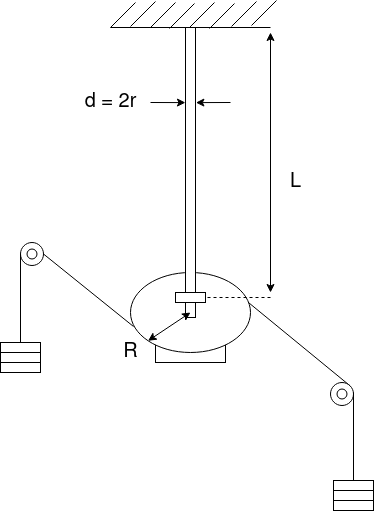
\includegraphics[width=0.4\textwidth]{images/young-twisting.drawio.png}
    \caption{Схема на уред за изследване на усукване}
    \label{fig:setup-twisting}
\end{figure}

На фиг. \ref{fig:setup-twisting} е представена принципна схема на уреда, чрез който ще изследваме деформацията при усукване. Устройството се състои от пръчка с дължина $L$ и радиус $r$, закрепена от едната страна неподвижно, а от другата за диск с радиус $R$. Около този диск преминава нишка, от двете страни на която могат да се закачат тежести. Закрепвайки тежести, дискът се отклонява от началното си положение, като по този начин пръчката се огъва. 

Вторият модул на еластичност пресмятаме по формула \ref{eq:phi-modulus}, където $M = 2m_igR$, а R е радиусът на диска. По получените данни, записани в таблица \ref{tbl:general}, пресмятаме и получаваме стойностите за втория модул на еластичност, които записваме в таблица \ref{tbl:summary-results}. На всяка итерация слагаме тежести с една и съща маса, но тъй като те с малко се различават, взимаме средната стойност между тях и ги записваме в колона $m_i$. Грешките изчисляваме по формула \ref{eq:second-modulus-err}.

\begin{equation}\label{eq:second-modulus-err}
    \Delta \Phi = \Phi \left(\frac{\Delta M}{M} + \frac{\Delta l}{l} + \frac{4\Delta R}{R} + \frac{\Delta \pi}{\pi} + \frac{\Delta (\Delta \phi)}{\phi}\right)
\end{equation}

\begin{table}[h]
\begin{center}
\begin{tabular}{|l|l|l|l|l|}\hline
N &m_{i1}, [kg] &m_{i2}, [kg] &\varphi_{i1}, [\degree] &\varphi_{i2}, [\degree] \\ \hline
0 &0 &0 &162.3 &161.3 \\ \hline
1 &0.0398 &0.03997 &165.3 &165.27 \\ \hline
2 &0.04 &0.04 &168 &167 \\ \hline
3 &0.05 &0.0499 &171 &169.9 \\ \hline
4 &0.04979 &0.04986 &174 &173 \\\hline
\end{tabular}
\caption{\label{tbl:general}Измерени стойности на ъглите и масите от двете страни на диска}
\end{center}
\end{table}

\begin{table}[h]
\begin{center}
\begin{tabular}{|l|l|l|l|l|}\hline
N &m_i, [kg] &\Delta \varphi, [\degree] &\Delta \varphi, [rad] & (\Phi + \Delta \Phi) \cdot 10^{9}, [Pa] \\ \hline
0 &0 &- &- &- \\ \hline
1 &0.0399 &3.485 &0.0608 &27.24928 \pm 3.3840 \\ \hline
2 &0.0799 &5.7 &0.0995 &33.3686 \pm 4.1044 \\ \hline
3 &0.0899 &8.65 &0.1510 &24.7535 \pm 3.0356 \\ \hline
4 &0.0998 &11.7 &0.2042 &20.3000 \pm 2.4853 \\ \hline
&&&& $\bar{\Phi}$ = 26.4179 \pm 3.2523 \\ \hline
\end{tabular}
\caption{\label{tbl:summary-results}Пресметнати стойности за средна стойност на двете маси m_i, средна стойност на диференциала на ъгъла спрямо началното положение \Delta \phi и втори модул на еластичност}
\end{center}
\end{table}

\section{Задача: Изчисляване на дирекционния момент D с една от стойностите за $\Phi$}
От таблица \ref{tbl:summary-results} получаваме $\bar{\Phi} = 26.4179 \pm 3.2523 GPa$. Дирекционният момент D и неговата грешка изчисляваме по формула \ref{eq:direction-moment}. Получаваме $D = 0.7920 \pm 0.1927 N.m$ 

\begin{equation}\label{eq:direction-moment}
    D = \frac{\pi R^4\Phi}{2l}, \Delta D = D\left(\frac{\Delta \pi}{\pi} + \frac{4\Delta R}{R} + \frac{\Delta \Phi}{\Phi} + \frac{\Delta l}{l}\right)
\end{equation}

\end{document}
